\chapter{Die Anwendung}
\section{Zeitplan Ansicht}

\begin{figure}[ht]
  \centering
  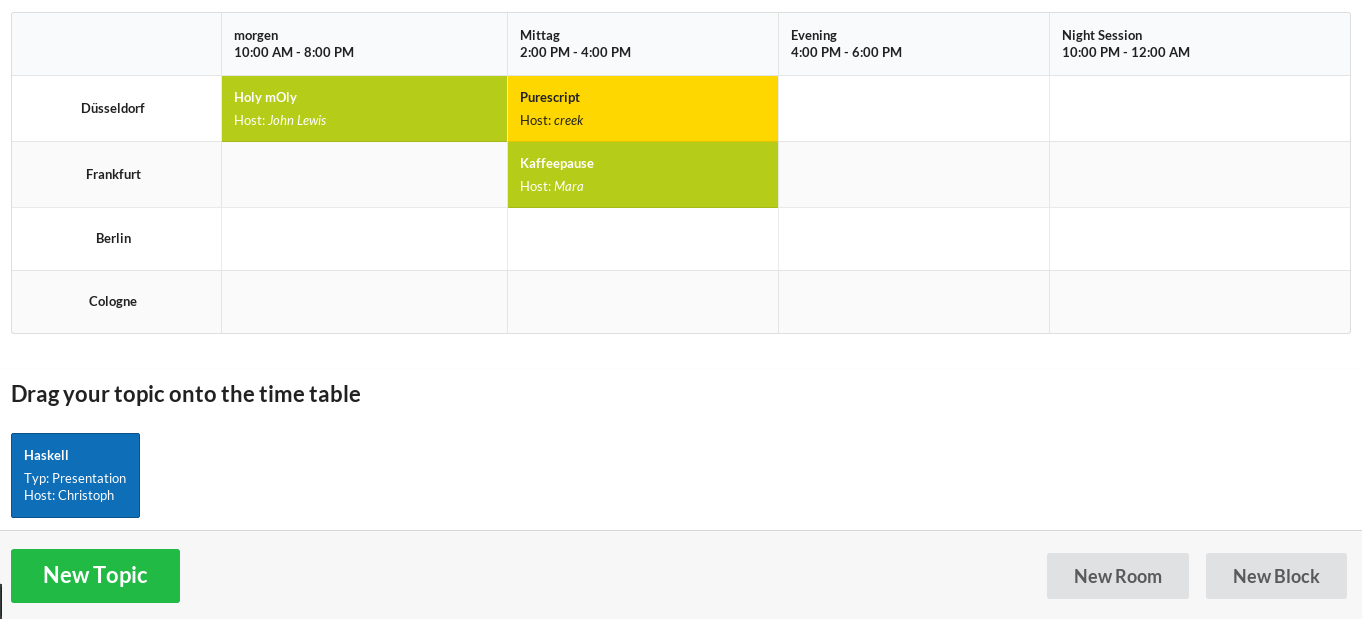
\includegraphics[width=\textwidth]{fig/timetable.png}
  \caption{Zeitplan}
\end{figure}

\subsection{Abschnitte}
Die Zeitplan Ansicht ist in drei visuelle Abschnitte eingeteilt.
\subsubsection*{Das Board}
Das Board ist eine zweidimensionale Matrix, bei der auf der X-Achse die
Zeitslots und auf der Y-Achse die Räume liegen. In den einzelnen Zellen der
Matrix befinden sich Themen die zur Zeit x in Raum y stattfinden.
\subsubsection*{Themenspeicher}
Im Themenspeicher befinden sich Themen die noch keinem Raum und Zeitslots
zugeordnet wurden.
\subsubsection*{Fußzeile}
In der Fußzeile befinden sich Knöpfe zum Anlegen von Räumen, Zeitslots und
Themen.
\subsection{Aktionen}
Auf der Zeitplan Ansicht wird die Planung und Organisation des Open Spaces
durchgeführt. Hierfür werden drei verschiedene Arten von Aktionen unterstützt.
\subsubsection*{Anlegen}
In der Zeitplan Ansicht lassen sich die Räume und Zeitslots der Veranstaltung
anlegen und anpassen. Weiterhin werden in dieser Ansicht neue Themen angelegt
und dem Board hinzugefügt. Das Anlegen der Räume, Zeitslots und Themen wird in
Popups mit den nötigen Angaben vorgenommen, die sich durch Klicks auf die
entsprechenden Knöpfe in der Fußzeile aufrufen lassen. Für neue Themen stehen
verschiedene Typen zur Verfügung:
\begin{itemize}
\item Diskussion -- Gelb
\item Präsentation -- Blau
\item Workshop -- Grün
\end{itemize}

\subsubsection*{Verschieben}
Neu angelegte Themen werden zunächst im Themenspeicher abgelegt und können dann
per Drag `n Drop auf das Board gezogen werden. Genauso können Themen auf dem
Board in andere Slots gezogen oder vom Board entfernt werden. Verschiebt man ein
Thema auf ein Feld das bereits belegt war, wird das vorige Thema in den
Themenspeicher gelegt und neue Thema dem Feld zugewiesen.

\subsubsection*{Entfernen}
Möchte man ein Thema vollständig löschen, erscheint, sobald man das Thema
angehoben hat, in der Fußzeile eine breiter Löschstreifen der durch ein
Mülltonnen Icon gekennzeichnet ist. Bewegt man ein Thema über diesen Streifen
leuchtet dieser rot auf und lässt man das Thema nun los wird es gelöscht.

Weiterhin können auch einmal erstellte Räume und Zeitslots wieder entfernt
werden. Bewegt man die Maus über die entsprechende Tabellenzeile im Tabellenkopf
oder in der ersten Tabellenspalte, erscheint ein X-Icon bei dessen Klick der
entsprechende Raum oder Zeitslot vom Board entfernt wird.
%%% Local Variables:
%%% mode: latex
%%% TeX-master: "../ai-projekt"
%%% End:
